\chapter{Preliminaries}


%\subsection{Notations and lemmas on mincuts}
Let $G=(V,E)$ be an undirected unweighted multigraph without self-loops. To contract (or compress) a set of vertices $U\subseteq V$ means to replace all vertices in $U$ by a single vertex $u$, delete all edges with both endpoints in $u$ and for every edge which has one endpoint in $U$, replace this endpoint by $u$. A graph obtained by performing a sequence of vertex contractions is called a {\em quotient} graph of $G$.


For any given $A,B\subset V$ such that $A\cap B=\emptyset$, we use $c(A,B)$ to denote the number of edges with one endpoint in $A$
and another in $B$. Overloading the notation, we shall use $c(A)$ for $c(A,\bar{A})$.

\begin{definition}[$(s,t)$-cut]
A subset of edges whose removal disconnects $t$ from $s$ is called an $(s,t)$-cut. An $(s,t)$-mincut is an $(s,t)$-cut of minimum cardinality. 
\label{def:(u,v)-cut}
\end{definition}

\begin{definition}[set of vertices defining a cut]
A subset $A\subset V$ is said to define an ($s,t$)-cut if $s\in A$ and $t\notin A$. The corresponding cut is denoted by cut$(A,\bar{A})$ or more compactly cut$(A)$.  
\label{def:set-definiting-a-cut}
\end{definition}

The following lemma exploits the undirectedness of the graph.
\begin{lemma}
Let $x,y,z$ be any three vertices in $G$. If $c_{x,y}>c$ and $c_{y,z}>c$, then $c_{x,z}>c$ as well. 
\label{lem:triangle-inequality}
\end{lemma}

When there is no scope of confusion, we do not distinguish between a mincut and the set of vertices defining the mincut. 
We now state a well-known property of cuts.
% \begin{lemma}[Submodularity of cuts]
% For any two subsets $A,B\subset V$, the following inequality holds.
% \[ c(A) +c(B) \ge c(A\cup B) + c(A\cap B) \]
% \label{lem:submodularity}
% \end{lemma}
\begin{lemma}[Submodularity of cuts]
For any two subsets $A,B\subset V$, ~
$ c(A) +c(B) \ge c(A\cup B) + c(A\cap B)$.
\label{lem:submodularity}
\end{lemma}


%The proof of the following lemma exploits just the property of a $(u,v)$-mincut.
\begin{lemma}
Let $S \subset V$ define an $(s,t)$-mincut with $s\in S$. For any subset $S'\subset V\setminus S$ with $v\notin S'$,
\[ 
c(S,S') \le c(S,V\setminus (S\cup S'))
\]
\label{lem:subset-property-of-min-cut}
\end{lemma}
\vspace{-10mm}
\section{Compact representation for all \texorpdfstring{$(s,t)$}{(s,t)}-mincuts}
Dinitz and Vainshtein \cite{DBLP:journals/siamcomp/DinitzV00} showed that there exists a quotient graph of $G$ that compactly stores all $(s,t)$-mincuts. This graph is called strip ${\cal D}_{s,t}$. The 2 node to which $s$ and $t$ are mapped in ${\cal D}_{s,t}$ are called the terminal nodes, denoted by ${\bf s}$ and ${\bf t}$ respectively. Every other node is called a non-terminal node. We now elaborate some interesting properties of the strip ${\cal D}_{s,t}$.
% by Dinitz and Vainshtein \cite{DBLP:journals/siamcomp/DinitzV00}

 Consider any non-terminal node $v$, and let $E_v$ be the set of edges incident on it in ${\cal D}_{s,t}$. There exists a unique partition, called {\em inherent partition}, of $E_v$ into 2 subsets of equal sizes. These subsets are called the 2 sides of the inherent partition of $E_v$. 
 %Dinitz and Vainshtein established the following very interesting property of this inherent partition.
 Interestingly, if we traverse ${\cal D}_{s,t}$ such that upon visiting any non-terminal node using an edge from one side of its inherent partition, the edge that we traverse while leaving it belong to the other side of the inherent partition, then no node will be visited again. Such a path is called a {\em coherent} path in ${\cal D}_{s,t}$. Furthermore, if we begin traversal from a non-terminal node $u$ along one side of its inherent partition and keep following a coherent path we are bound to reach the terminal ${\bf s}$ or terminal ${\bf t}$. So the two sides of the inherent partitions can be called side-${\bf s}$
 and side-${\bf t}$ respectively.
It is because of these properties
that the strip ${\cal D}_{s,t}$ can be viewed as an undirected analogue of a directed acyclic graph with a single source and a single sink. 

A cut in the strip ${\cal D}_{s,t}$ is said to be a \textit{transversal} if each coherent path in ${\cal D}_{s,t}$ intersects it at most once. The following lemma provides the key insight for representing all $(s,t)$-mincuts through the strip ${\cal D}_{s,t}$.
\begin{lemma}[\cite{DBLP:journals/siamcomp/DinitzV00}]
    $A\subset V$ defines a $(s,t)$-mincut if and only if $A$ is a transversal in ${\cal D}_{s,t}$.
    \label{lem:mincut-transversal}
\end{lemma}

We now state the following two lemmas that can be viewed as a corollary of Lemma \ref{lem:mincut-transversal}.

\begin{lemma}
A $(s,t)$-mincut contains a set of edges $E_y$ incident on vertex $y$ if and only if all edges in $E_y$ must belong to the same side of the inherent partition of the node containing $y$ in strip ${\cal D}_{s,t}$.
\label{lem:E_y-edges-same-side}
\end{lemma}

\begin{lemma} 
If $A\subset V$ defines a $(s,t)$-mincut with $s\in A$, then $A$ can be merged with the terminal node ${\mathbf s}$ in ${\cal D}_{s,t}$ to get the strip ${\cal D}_{A,t}$ that stores all those $(s,t)$-mincuts that enclose $A$.
\label{lem:strip-A}
\end{lemma}


Consider any non-terminal node $x$. Let ${\cal R}_s(x)$ be the set of all the nodes $y$ in ${\cal D}_{s,t}$ that are reachable from $x$ through coherent paths that originate from the side-${\bf s}$ of the inherent partition of $x$ -- notice that all these paths will terminate at ${\bf s}$. 
It follows from the construction that ${\cal R}_s(x)$ defines a transversal in
${\cal D}_{s,t}$. We call ${\cal R}_s(x)$ the \textit{reachability cone} of $x$ towards $s$. 
The $(s,t)$-mincut defined by ${\cal R}_s(x)$ is the nearest mincut from $\{s,x\}$ to $t$. 
Interestingly, each transversal in ${\cal D}_{s,t}$, and hence each $(s,t)$-mincut, is a union of the reachability cones of a subset of nodes of ${\cal D}_{s,t}$ in the direction of $s$. We now state the following Lemma that we shall crucially use.

\begin{lemma}[\cite{DBLP:journals/siamcomp/DinitzV00}]
If $x_1,\ldots, x_k$ are any non-terminal nodes in strip ${\cal D}_{s,t}$,  the union of the reachability cones of $x_i$'s in the direction of ${\mathbf s}$ defines the nearest mincut between $\{s, x_1,\ldots, x_k\}$ and $t$.
\label{lem:reachability-cones}
\end{lemma} 


\section{Compact representation for all global mincuts} \label{appendix:cactus}

Let $c_V$ denote the value of the global mincut of the graph $G$.
Dinitz, Karzanov, and Lomonosov \cite{DL76} showed that there exists a graph ${\cal H}_V$ of size $O(n)$ that compactly stores all global mincuts of $G$. 
%In order to maintain the distinction between the two graphs,
Henceforth, we shall use nodes and structural edges for vertices and edges of ${\cal H}_V$ respectively. There exists a projection mapping $\pi:V(G)\rightarrow V({\cal H}_V)$ assigning a vertex of graph $G$ to a node in graph ${\cal H}_V$. In this way, any cut $(A,{\bar A})$ in cactus ${\cal H}_V$ is associated to a cut $(\pi^{-1}(A),\pi^{-1}(\bar A))$ in the original graph $G$.
The graph ${\cal H}_V$ has a nice tree-like structure with the following properties.
\begin{enumerate}
    \item Any two distinct simple cycle of ${\cal H}_V$ have at most a node in common. This is equivalent to the property that each structural edge of ${\cal H}_V$ belongs to at most one simple cycle. Each cut in ${\cal H}_V$ either corresponds to a tree edge or a pair of cycle edges in the same cycle.
    \item If a stuctural edge belongs to a simple cycle, it is called a \textit{cycle edge} and its weight is $\frac{c_V}{2}$. Otherwise, the structural edge is called a \textit{tree edge} and its weight is $c_V$.
    \item For any cut in the cactus ${\cal H}_V$, the associated cut in graph $G$ is a global mincut. Moreover, any global mincut in $G$ must have at least one associated cut in ${\cal H}_V$.
\end{enumerate}

Let $\nu$ and $\mu$ be any two nodes in the cactus ${\cal H}_V$. If they belong to the same cycle, say $c$, there are two paths between them on the cycle $c$ itself - their union forms the cycle itself. Using the fact that any two cycles in  ${\cal H}_V$ can have at most one common node, it can be seen that these are the only paths between $\nu$ and $\mu$. Using the same fact, if $\nu$ and $\mu$ are two arbitrary nodes in the cactus, there exists a unique path of cycles and tree edges between these two nodes. Any global mincut that separates $\nu$ from $\mu$ must correspond to a cut in this path.

\subsection{Construction of $(s,t)$-strip from cactus}
\label{sec:construction-strip-cactus}
Suppose $s,t \in V$ are two vertices such that $c_{s,t}$ is same as the global mincut value. 
So, each transversal of strip ${\cal D}_{s,t}$ corresponds to a global mincut that separates $s$ and $t$. Recall that cactus ${\cal H}_V$ stores all global mincuts. So we just need to contract it suitably so that only those cuts remain that separate $s$ and $t$. For this purpose,
we compute the path of cycles and tree edges between the nodes corresponding to $s$ and $t$ respectively. We compress each of the subcactus rooted to this path to a single vertex. The resultant graph we obtain will be the strip ${\cal D}_{s,t}$. The inherent partition of all the non-terminal units can be determined using the endpoints of the edges in the path.

\subsection{Tree representation for cactus}

%  Let $G=(V,E)$ be an undirected graph, $S\subseteq V$ be the Steiner set of vertices and let ${\cal H}_S$ be the cactus graph storing all bunches of Steiner mincuts. 

We shall now show that ${\cal H}_V$ can be represented as a tree structure. This tree structure was also used by Dinitz and Westbrook in \cite{DBLP:journals/algorithmica/DinitzW98}. This representation will simplify our analysis on the cactus.

We now provide the details of the graph structure $T({\cal H}_V)$ that represents ${\cal H}_V$. The vertex set of $T({\cal H}_V)$ consists of all the cycles and the nodes of the cactus. For any node $\nu$ of the cactus ${\cal H}_V$, let $v(\nu)$ denote the corresponding vertex in $T({\cal H}_V)$. Likewise, for any cycle $\pi$ in the cactus, let $v(\pi)$ denote the corresponding vertex in $T({\cal H}_V)$. We now describe the edges of  $T({\cal H}_V)$. Let $\nu$ be any node of ${\cal H}_V$. Suppose there are $j$ cycles - $\pi_1,\ldots,\pi_j$ that pass through it. We add an edge between $v(\nu)$ and $v(\pi_i)$ for each $1\le i\le j$. Lastly, for each vertex $\nu(\pi)$ in $T{({\cal H}_V)}$ we store all its neighbours in the order in which they appear in the cycle $\pi$ in ${\cal H}_V$. This is done to ensure that information about the order of vertices in each cycle is retained. This complete the description of $T({\cal H}_V)$. For a better understanding, the reader may refer to Figure \ref{fig:transform-cactus-to-tree} that succinctly depicts the transformation carried out at a node $\nu$ of the cactus graph to build the corresponding graph structure $T({\cal H}_V)$. 

The fact that the graph structure $T({\cal H}_V)$ is a tree follows from the property that any two cycles in a cactus may have at most one vertex in common. Let us root $T({\cal H}_V)$ at any arbitrary vertex, say $v(\nu)$, for some node $\nu$ of ${\cal H}_V$. Since each cycle in ${\cal H}_V$ has at least 3 vertices, so each vertex corresponding to a cycle of ${\cal H}_V$ will have at least 2 children each corresponding to distinct nodes of ${\cal H}_V$. This also shows that the number of cycles in ${\cal H}_V$ is at most half of the number of nodes in ${\cal H}_V$. Hence, the size of $T({\cal H}_V)$ is of the order of the number of nodes of ${\cal H}_V$. 

\begin{figure}
\centering
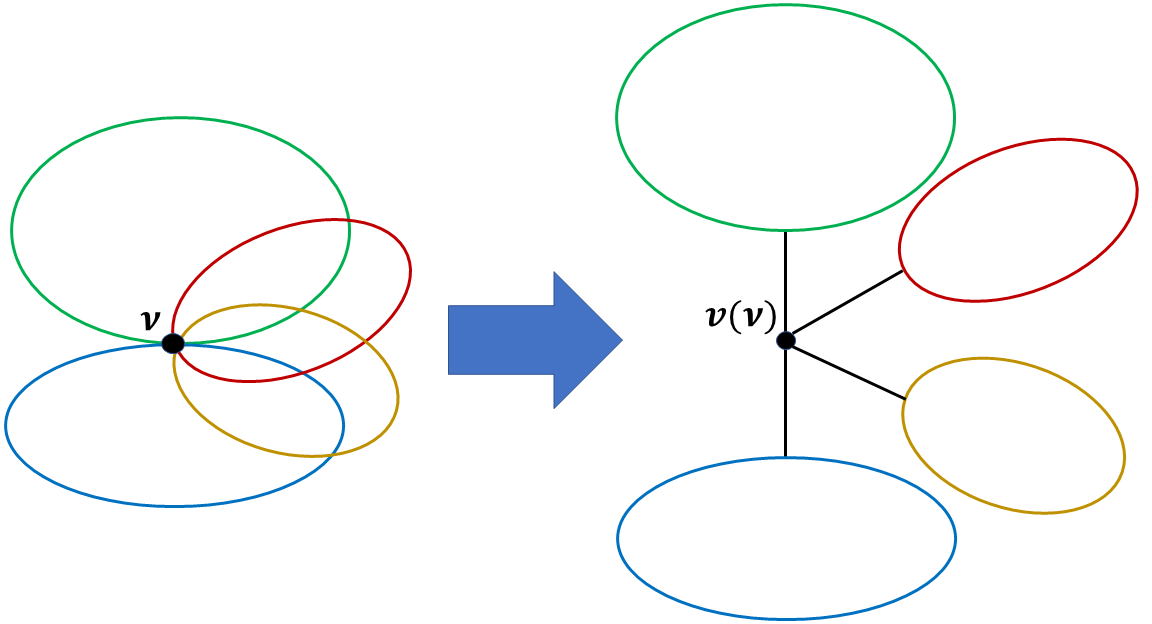
\includegraphics[width=0.6\textwidth]{src/images/Cactus-transformation.png}
    \caption{Transformation of cactus ${\cal H}_V$ to the tree $T({\cal H}_V)$.}
\label{fig:transform-cactus-to-tree}
\end{figure}

We know that if $\nu$ and $\mu$ are two nodes in the cactus, there exists a unique path of cycles and tree edges between them. It follows from the construction of $T({\cal H}_V)$ that the unique path between the vertices $v(\nu)$ and $v(\mu)$ captures the same path. Thus we state the following lemma.

\begin{lemma}
Let $\nu,\mu$ be any two arbitrary nodes in the cactus 
${\cal H}_V$. The unique path between $v(\nu)$ and $v(\mu)$ in $T({\cal H}_V)$ concisely captures all
paths between $\nu$ and $\mu$ in ${\cal H}_S$.
\label{lem:path-in-T(H_S)}
\end{lemma}

% Let $\nu$ and $\mu$ be any two nodes in skeleton ${\cal H}_S$. If they belong to the same cycle, say $c$, there are two paths between them on the cycle $c$ itself - their union forms the cycle itself. Using the fact that any two cycles in  ${\cal H}_S$ can have at most one common node, it can be seen that these are the only paths between $\nu$ and $\mu$. Using the same fact, if $\nu$ and $\mu$ belong to different cycles, there exists a unique sequence of alternating cycles and nodes $\langle \nu_1,c_1,\ldots,\nu_r,c_r,\nu_{r+1}\rangle $ satisfying the following 2 properties. \begin{itemize}
%     \item $\nu_1=\nu$, $\nu_{r+1}=\mu$, and for each $1< i\le r$, $\nu_i$ is the unique node common to $c_{i-1}$ and $c_i$.
%     \item Each path between $\nu$ and $\mu$ can be seen as a sequence $\langle p_1,\ldots p_r\rangle$ such that $p_i$ is a path between $\nu_i$ and $\nu_{i+1}$ on cycle $c_{i}$.
% \end{itemize}
% It follows from the construction of $T({\cal H}_S)$ that $\langle v(\nu_1),v(c_1),\ldots,v(\nu_r),v(c_r),v(\nu_{r+1})\rangle$ is the path between $v(\nu)$
% and $v(\mu)$. 
% Thus we can state the following lemma.
% \begin{lemma}
% Let $\nu,\mu$ be any two arbitrary nodes in the cactus 
% ${\cal H}_S$. The unique path between $v(\nu)$ and $v(\mu)$ in $T({\cal H}_S)$ concisely captures all
% paths between $\nu$ and $\mu$ in ${\cal H}_S$.
% \label{lem:path-in-T(H_S)}
% \end{lemma}

We root the tree $T({\cal H}_V)$ at any arbitrary vertex and augment it suitably so that it can answer any LCA query in $\mathcal O(1)$ time using \cite{DBLP:journals/jal/BenderFPSS05}. Henceforth, we shall use skeleton tree $T({\cal H}_S)$ to denote this data structure.

\section{Compact representation for all Steiner mincuts} \label{subsec:connectivity-carcass}

% Let $G=(V,E)$ be an undirected unweighted graph and $S\subseteq V$ be a subset (Steiner set) of its vertices. 
Dinitz and Vainshtein \cite{DBLP:conf/stoc/DinitzV94} designed a data structure $\mathfrak{C}_S = ({\cal F}_S,{\cal H}_S, \pi_S)$ that stores all the Steiner mincuts for a Steiner set $S\subseteq V$ in the graph. We present a summary of this data structure.

This data structure can be seen as a generalization of two already discussed data structures,
~(i) strip ${\cal D}_{s,t}$ storing all $(s,t)$-mincuts, and
~(ii) cactus graph ${\cal H}_V$ storing all global mincuts.

Two $S$-mincuts are said to be equivalent if they divide the Steiner set $S$ in the same way. The equivalence classes thus formed are known as the \textit{bunches}. Similarly, two vertices are said to be equivalent if they are not separated by any Steiner mincut. The equivalence classes thus formed are known as \textit{units}. A unit is called a \textit{Steiner unit} if it contains at least a Steiner vertex.

Let $(S_B,{\bar S_B})$ be the $2-$partition of Steiner set induced by a bunch $\cal B$. If we compress all vertices in $S_B$ to $s$ and all vertices in ${\bar S_B}$ to $t$, the strip ${\cal D}_{s,t}$ will store all cuts in ${\cal B}$. We shall denote this strip by ${\cal D}_{\cal B}$. Any such strip has the following property -- if two non-terminals nodes of two strips intersect at even one vertex then these nodes coincide and the inherent partitions of these nodes in both strips coincide as well.

The first component of the connectivity carcass is the \textit{flesh graph} ${\cal F}_S$ which is a generalization of the strip. This graph is a quotient graph of graph $G$. The vertices of ${\cal F}_S$ can be obtained by contracting each unit of $G$ to a single vertex. Thus, we denote the vertices of ${\cal F}_S$ simply by units. In addition to it, each unit of ${\cal F}_S$ is assigned a $2-$partition known as the \textit{inherent partition} on the set of edges incident on it. Any unit that appears as a non-terminal in the strip corresponding to some bunch is called a \textit{stretched unit}. Otherwise, it is called a \textit{terminal unit}. 
% Another distinction between these two units follows from the two observations made on strip corresponding to a bunch mentioned above. 
The inherent partition assigned to a stretched unit consists of two sets of equal cardinality. On the other hand, inherent partition assigned to a terminal unit is a trivial partition (one of the set is empty). Note that all Steiner units are terminal units but the reverse is not true.
% The concept of reachability is slightly modified in ${\cal F}_S$. Whenever we say that a unit $u$ is reachable from unit $u'$, it means that there exists a coherent path between $u$ and $u'$. A \textit{coherent path} refers to a sequence of units and edges in flesh $(u_1,e_1,u_2,e_2,\ldots,u_k)$ such that any $e_i$ is incident on $u_{i-1}$ and $u_i$ and for any $u_i$ $e_{i-1}$ and $e_i$ lie in different side of the inherent partition. The structure of the flesh graph implies that it is not possible for a coherent path to start and finish at a single unit and hence, ${\cal F}_S$ is in a sense acyclic. A \textit{transversal} refers to a $2-$partition of units such that any coherent path intersects it at most once. It can be shown that each transversal in the flesh ${\cal F}_S$ corresponds to a Steiner mincut.
The concept of reachability in ${\cal F}_S$ is similar to the strip. Whenever we say that a unit $u$ is reachable from unit $u'$, it means that there exists a coherent path between $u$ and $u'$. The structure of ${\cal F}_S$ is such that a coherent path cannot start and finish at a single unit and hence, ${\cal F}_S$ is in a sense acyclic. There is a one-to-one correspondence between transversals in ${\cal F}_S$ and Steiner mincuts in $G$.

The second component of the connectivity carcass, skeleton ${\cal H}_S$, is a cactus graph. 
To avoid confusion with the original graph, the vertices and edges of the skeleton will be referred to as nodes and structural edges respectively. 
% A structural edge in the skeleton is a tree-edge if it is not part of a cycle, otherwise, it is a cycle-edge. 
% If $c_S$ is the value of the Steiner mincut, then each tree-edge is assigned weight $c_S$ and each cycle-edge is assigned weight $\frac{c_S}{2}$. 
Each terminal unit of ${\cal F}_S$ is mapped to a node in the skeleton ${\cal H}_S$ by projection mapping ${\pi}_S$. A stretched unit on the other hand is mapped to a set of edges corresponding to a proper path in ${\cal H}_S$ by ${\pi}_S$. A \textit{proper path} in the skeleton refers to an alternating sequence of nodes and structural edges $(\nu_1,\epsilon_1,\nu_2,...,\nu_k)$ such that $\epsilon_i$ is incident on $\nu_{i-1}$ and $\nu_i$ and it intersects each cycle of the skeleton at at most one structural edge. 
% A \textit{subbunch} is a subset of a bunch that can be represented by a strip. 
All the bunches can be stored in a skeleton ${\cal H}_S$ in the form of subbunches (disjoint subsets of a bunch). Each cut in skeleton corresponds to a subbunch. The strip ${\cal D}_{\cal B}$ corresponding to this subbunch $\cal B$ can be obtained as follows. Let the cut in the skeleton separates it into two subcactuses ${\cal H}_S(\cal B)$ and ${\bar {\cal H}_S(\cal B)}$. If $P(\nu_1,\nu_2)$ be the path in the skeleton to which a unit $u$ is mapped, it will be placed in ${\cal D}_{\cal B}$ as follows.
\begin{itemize}
    \item If both $\nu_1$ and $\nu_2$ lie in ${\cal H}_S(\cal B)$ (or ${\bar {\cal H}_S(\cal B)}$) $u$ is contracted in source (or sink).
    \item Otherwise, $u$ is kept as a non-terminal unit.
\end{itemize}


Now we discuss an important property between the reachability of a stretched unit $u$ and the proper path to which it is mapped in the skeleton ${\cal H}_S$.

\begin{lemma}[\cite{DBLP:conf/soda/DinitzV95}]
Let $u$ be a stretched unit and $u'$ be any arbitrary unit in the flesh ${\cal F}_S$ and $\pi_S(u) = P(\nu_1,\nu_2)$, $\pi_S(u') = P(\nu_3,\nu_4)$. If $u'$ is reachable from $u$ in direction $\nu_2$, then both these paths are extendable to a larger proper path with $P(\nu_1,\nu_2)$ as the initial part and $P(\nu_3,\nu_4)$ as the final part.
\label{lem:path-extendable}
\end{lemma}

\begin{lemma}[\cite{DBLP:conf/stoc/DinitzV94}]
\label{lem:strip-from-carcass}
Let $s,t \in S$ such that $c_{s,t}=c_S$. Given the connectivity carcass ${\mathfrak C}_S$ storing all Steiner mincuts, the strip ${\cal D}_{s,t}$ can be constructed in time linear in the size of flesh graph.
\end{lemma}

The size of flesh ${\cal F}_S$ is ${\cal O}(\min(m,\tilde{n}c_S))$ where $\tilde{n}$ is the number of units in ${\cal F}_S$. The size taken by skeleton is linear in the number of Steiner units. Thus, overall space taken by the connectivity carcass is ${\cal O}(\min(m,\tilde{n}c_S))$.